\documentclass[10pt]{article}
\usepackage[utf8]{inputenc}
\usepackage[T1]{fontenc}
\usepackage{amsmath}
\usepackage{amsfonts}
\usepackage{amssymb}
\usepackage[version=4]{mhchem}
\usepackage{stmaryrd}
\usepackage{graphicx}
\usepackage[export]{adjustbox}
\graphicspath{ {./images/} }

\title{Università di Catania 
 Corso di Laurea in Fisica 
 Compito scritto di Fisica Generale I 
 M.G. Grimaldi - A. Insolia }

\author{}
\date{}


\begin{document}
\maketitle
Catania, 22 Giugno 2022

Per la prova in itinere ( 2 ore) svolgere i problemi: \(3,4,5\)

Per la prova completa ( 3 ore) svolgere i problemi: \(1,2,3,4\)

\section{Problema n.1}
Un corpo (puntiforme) di massa \(m=3.00 \mathrm{~kg}\) viene lanciato orizzontalmente con una velocità \(v_{0}\), diretta come in figura, su di un piano privo di attrito. Come si vede dalla figura, procedendo verso destra il corpo raggiunge una lastra (inizialmente in quiete) anch'essa libera di muoversi senza attrito. La lastra ha lunghezza \(\mathrm{l}=2.00 \mathrm{~m}\) e massa \(M=20.0 \mathrm{~kg}\). Quando il corpo scivola sulla lastra risente di un attrito dinamico con \(\mu_{\mathrm{k}}=0.500\). Sapendo che dopo esservi salito il corpo raggiunge il centro della lastra (rimanendo in quiete rispetto ad essa), determinare:

a) il valore di \(v_{0}\); [risultato: \(3.36 \mathrm{~m} / \mathrm{s}\) ]

b) la velocità finale del sistema lastra+corpo; [risultato: \(0.44 \mathrm{~m} / \mathrm{s}\) ]

c) l'energia dissipata nell'intero processo. [risultato: \(14.7 \mathrm{~J}\) ]

\begin{center}
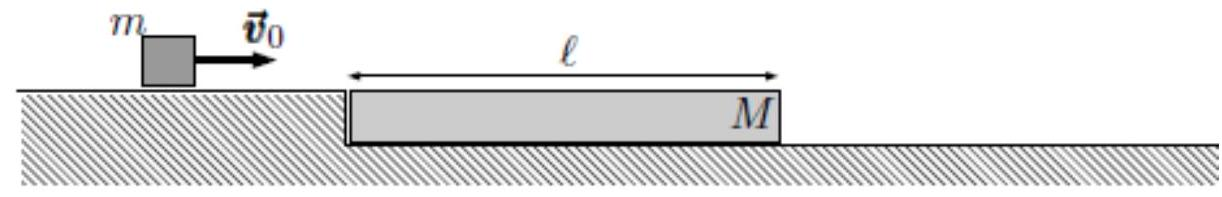
\includegraphics[max width=\textwidth]{2023_05_14_871182cc3780357c06a3g-1(1)}
\end{center}

\section{Problema n.2}
Come schematizzato in figura, si abbia una sbarra rigida sottile, di lunghezza \(\mathrm{I}=2.00 \mathrm{~m}\) e massa \(\mathrm{m}\), disposta in un piano verticale. La sbarra può ruotare liberamente intorno ad un perno orizzontale passante per un suo estremo. La sbarra viene liberata (da ferma) quando forma un angolo iniziale \(\theta_{0}\) con l'orizzontale (vedi figura); quando la sbarra raggiunge la verticale il suo estremo inferiore urta elasticamente un corpo di massa \(\mathrm{m} / 2\) posto in quiete in quella posizione. Trascurando ogni forma di attrito e sapendo che dopo l'urto il corpo puntiforme parte verso sinistra con una velocità \(\mathrm{v}_{\mathrm{f}}=6.00 \mathrm{~m} / \mathrm{s}\), determinare:

a) I'angolo \(\theta_{0}\) da cui è stata lasciata andare la sbarra; [risultato: \(-2.54^{\circ}\) ]

b) l'angolo massimo (dalla verticale) che raggiunge la sbarra dopo l'urto. [risultato: \(15.9^{\circ}\) ]

\begin{center}
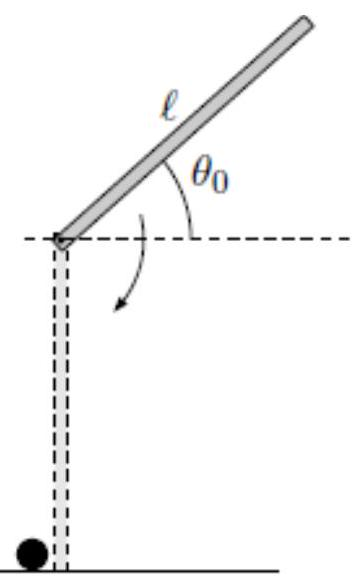
\includegraphics[max width=\textwidth]{2023_05_14_871182cc3780357c06a3g-1}
\end{center}

\section{Problema n.3}
Un recipiente è costituito da un cilindro verticale di diametro \(D=9.0 \mathrm{~cm}\) sul quale è innestato un tubo orizzontale di diametro \(\mathrm{d}=3.0 \mathrm{~cm}\) ad una distanza \(\mathrm{I}=5 \mathrm{~cm}\) dal fondo del cilindro. All' altro estremo del tubo orizzontale viene messo un tappo (vedi figura) ed il recipiente viene riempito di acqua fino all' altezza \(h=50 \mathrm{~cm}\).

a) Si determini la velocità di uscita dell'acqua quando viene rimosso il tappo. Si noti che d non è trascurabile rispetto a D. [risultato \(2.98 \mathrm{~m} / \mathrm{s}\) ]

b) A che distanza dal tubo l'acqua in uscita tocca il piano? [risultato: \(0.3 \mathrm{~m}\) ]

\begin{center}
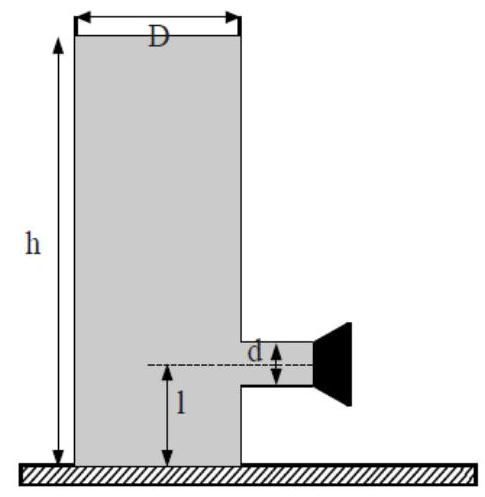
\includegraphics[max width=\textwidth]{2023_05_14_871182cc3780357c06a3g-2}
\end{center}

\section{Problema n.4}
Un quantità \(\mathrm{n}=1.50\) mol di un gas ideale biatomico segue il ciclo reversibile schematizzato in figura costituito dalle seguenti trasformazioni: \(1 \rightarrow 2\) isobara; \(2 \rightarrow 3\) isocora; \(3 \rightarrow 1\) trasformazione corrispondente al segmento rettilineo che unisce gli stati 3 e 1. Pressione e temperatura dello stato 1 sono \(p_{1}=3.00\) atm e \(T_{1}=200 \mathrm{~K}\); per i volumi e le pressioni degli altri stati è \(\mathrm{V}_{2}=\mathrm{V}_{3}=2 \mathrm{~V}_{1}\) e \(\mathrm{p}_{3}=\) \(\mathrm{p}_{1} / 3\).

Determinare:

a) il volume occupato dal gas nello stato 1 e le sue temperature negli stati 2 e 3; [risultati: 8.21 \(\left.\mathrm{dm}^{3}, 400 \mathrm{~K}, 133 \mathrm{~K}\right]\)

b) il lavoro compiuto dal gas nell'intero ciclo; [risultato: \(831 \mathrm{~J}\) ]

c) la variazione di entropia subita dallo stesso nella trasformazione \(3 \rightarrow 1\). [risultato: \(4.00 \mathrm{~J} / \mathrm{K}\) ]

\begin{center}
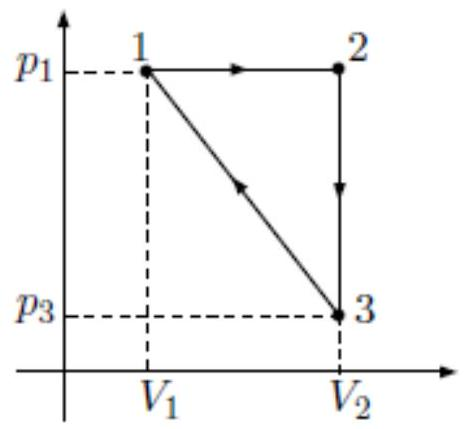
\includegraphics[max width=\textwidth]{2023_05_14_871182cc3780357c06a3g-2(1)}
\end{center}

\section{Problema n.5}
Un pezzetto di ghiaccio di massa \(\mathrm{m}\) e alla temperatura di \(T_{1}=250 \mathrm{~K}\) viene immerso in \(\mathrm{m}_{2}=60 \mathrm{~g}\) di acqua a temperatura di \(T_{2}=330 \mathrm{~K}\). Se il sistema è contenuto in un recipiente a pareti adiabatiche:

a) si determini per quali valori della massa m il pezzetto di ghiaccio fonde completamente; [risultato: minore o uguale a \(37.8 \mathrm{~g}\) ] b) calcolare la temperatura di equilibrio del sistema se la massa del cubetto di ghiaccio vale \(35 \mathrm{~g}\). [risultato: \(309.1 \mathrm{~K}\) ]

II calore specifico del ghiaccio vale \(\mathrm{c}_{\mathrm{g}}=2051 \mathrm{~J} / \mathrm{KgK}\), il calore specifico dell'acqua vale \(\mathrm{c}_{\mathrm{a}}=4186.8\) \(\mathrm{J} / \mathrm{KgK}\) ed il calore latente di fusione del ghiaccio è pari a \(\lambda_{f}=3.3 \times 10^{5} \mathrm{~J} / \mathrm{Kg}\).


\end{document}